\chapter{A SC FILTER FOR ARBITRARY WEIGHTING FUNCTION SYNTHESIS}
\label{chapter:filter}
\hyphenation{topology simplicity}
\section{Introduction}

%In particle physics experiments, where the results from the collisions are inferred from the measurement of electric charge in various sets of detectors \citep{gatti101,radeka101}, noise sets a fundamental limit for the charge measurement resolution \citep{degeronimo102}. In such experiments, the typical detector \mbox{front-end} circuit comprises a \mbox{charge-sensitive} amplifier (CSA) and a filter, often referred to as pulse shaper. The former is used to convert the input charge signal, coming from the detector electrodes, into a voltage signal, and is responsible for most of the noise present in the readout circuit signal path \citep{degeronimo101,degeronimo102}. The filter is used to convert the voltage signal at the CSA output into a shaped voltage pulse, in order to maximize the \mbox{signal-to-noise} ratio (SNR) at the measurement time.  

%A current trend on particle physics instrumentation is to implement this filter in the discrete time domain, which allows to synthesize weighting functions (WFs) with virtually any shape, producing near-optimum filters. In \citep{diego101} a novel mathematical framework for a design-oriented analysis of discrete-time filters was presented. One of the greatest benefits of this framework is that it allows to easily compute the optimal discrete-time filter that maximize the SNR in a typical detector front-end circuit, a difficult task to achieve using the traditional methods intended for continuous-time networks. In this work, a generic filter designed to be flexible enough to synthesize arbitrary weighting functions is presented, 

One of the greatest benefits of the mathematical framework presented in \citep{avila101} is that it allows to easily find the optimal discrete-time filter that minimizes the noise of a typical detector front-end circuit, a difficult task to undertake using the traditional methods for continuous-time networks. The filter presented in this chapter is designed to be flexible enough to synthesize arbitrary weighting functions with an adequate resolution. Therefore, it could be used to synthesize the optimal filter described above. The filter is a prototype of the front-end filter for the Bean V2, which was introduced in Chapter~\ref{chapter:problem}. Hence, the main specifications are derived from the Bean specifications. Also, power, noise and size budgets of the referred IC are taken as constraints.

There are two common options for implementing the required filter. The simplest is to digitize the CSA output directly with a fast analog-to-digital converter (ADC)  - $N$ times faster than the typical used ADC, with $N$ the number of desired samples - and then process the samples in the digital domain, whereas the other option is to use a custom \mbox{switched-capacitor} (SC) network as a filter, without changing the ADC requirements. Considering the Bean timing constraints, the former option is not feasible, given that such fast ADC would exceed the available power and size budgets. Hence, the SC solution was finally chosen.


\section{System-Level Design}
As mentioned in the previous Chapter, to synthesize arbitrary weighting functions the front-end filter should be designed to have a  discrete-time transfer function $F(z)$ given by
\begin{equation}
F(z) = \sum_{j=0}^{N-1}a_{N-j} \hspace{0.1em}z^{-j} \label{eq:filter_tf}
\end{equation}
where $a_i$ are the filter gain coefficients and $N$ is the filter length. Fig.~\ref{fig:filter_post} shows a simplified circuit diagram of a fully-differential SC integrator designed to implement $F(z)$. Some control logic and switches have been purposely omitted.

The filter has two phases of operation. During the sampling phase, $\phi_1$, the input voltage charges  both $C_S$ capacitors. During the amplification phase, $\phi_2$, the OTA input virtual short circuit forces charge from capacitors $C_S$ to be transferred to capacitors $C_F$. Thus, at the end of $\phi_2$, the filter output voltage is equal to its value in the previous cycle, plus $C_S V_i/C_F$. Also, an early version of $\phi_1$, $\phi_{1e}$, is used in the sampling phase to implement Bottom-Plate Sampling \citep{haigh101}, a technique used to reduce the charge injection from switches.

In this configuration, the filter instantaneous gain is given by the ratio of the capacitors $C_S$ and $C_F$.  Considering that in order to obtain arbitrary coefficients the filter gain must be programmable, either $C_S$ or $C_F$ should be implemented with a variable capacitor. For simplicity, capacitor $C_S$ was selected for this purpose. The OTA input multiplexers are used to swap the OTA inputs, and therefore, to invert the sign of the filter gain. The OTA output common-mode level is set by the OTA's internal common-mode feedback (CMFB) circuit, whereas the input common-mode level is set by the external reference $V_\textit{icm}$. The OTA output multiplexers are used to bypass the filter for the SDT operation mode and for diagnostic purposes.


\begin{figure}[!t]
	\centering
	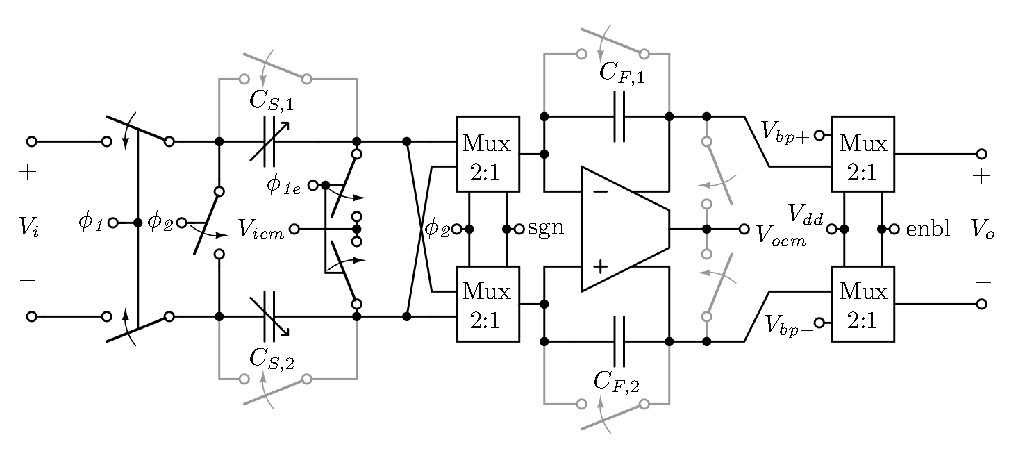
\includegraphics[width=6in]{./Figures/Filter/filter_post.eps}
	\caption{Simplified filter schematic. Reset switches are depicted in gray.}\label{fig:filter_post}
\end{figure}

\subsection{Filter Specifications}

Table \ref{tab:filter_specs} summarizes the filter specifications derived from the Bean specifications (Table \ref{tab:bean_specs}). Also, the CSA output specifications and the ADC input specifications were taken into account. The sampling frequency is $51.95\,\text{MHz}$. Thus, each integration subcycle is $19.25\,\text{ns}$ long. Since each subcycle involves two phases, sampling and holding, each phase has only $9.625\,\text{ns}$ for settling. Considering this time, to assure a dynamic error of $0.1\,\%$ (to meet the dynamic range specification) the amplifier must have a \mbox{worst-case} \mbox{closed-loop} bandwidth of $f_u = 118\,\text{MHz}$ (without considering slew-rate regime). Also, a static error of $0.1\,\%$ is required, which implies an OTA open-loop gain of at least $60\,\text{dB}$. 

\begin{table}[!t]
	\begin{center}
		\begin{tabular}{|l|l|}\hline
			{\bf Specification} & {\bf Value} \\ \hline\hline
			Modes of operation & SDT and DCal \\ \hline
			Input swing & 0.9 V or close \\ \hline
			Output swing & 1 V or close \\ \hline
			Dynamic range & 10 bits \\ \hline
			Gain resolution & 6 bits (7.8 mV/V - 0.5 V/V) \\ \hline
			Noise budget & $1.25\times Q_n^2$ \\ \hline
			Operation speed & $51.95\,\text{MHz}$ \\ \hline
			Power consumption & Minimize\\\hline
		\end{tabular}
		\vspace*{5pt}
		\caption{Filter specifications summary, where $Q_n^2$ is the readout ADC quantization noise.}\label{tab:filter_specs}
	\end{center}
\end{table}

%Besides the specifications required to implement arbitrary weighting functions, 

%
%In a SC integrator the noise should be analyzed at the two clock phases and then by added
%
%After $N$ integration cycles and assuming an arbitrary $C_S$ at each cycle, the contribution from noise sampled at $\phi_1$ can be computed as
%\begin{equation}
%\overline{V_{\phi_1}^2} = 2 kT \sum_{i=1}^{N} \frac{1}{C_{F_i}}\left(1 + \frac{C_S}{C_{F_i}}\right)
%\end{equation}
%
%In a proper design, switches resistance will be much smaller than $1/\beta g_\textit{m,eff}$, so noise contribution at $\phi_2$ can be assumed dominated by OTA noise. In a one stage OTA
%
%\begin{equation}
%\overline{V_{\phi_2}^2} = \frac{2 N_f kT}{g_\textit{meff}} \sum_{i=1}^{N} \frac{1}{\beta_i C_{Ltot_i}}
%\end{equation}
%
%where $N_f$ is a noise factor dependent on the OTA topology, for a recycling folded cascode
%
%\begin{equation}
%N_f \approx \left(1+\frac{g_{mf}}{g_{meff}}+\frac{g_{ml}}{g_{meff}}\right)
%\end{equation}
%
%
%In a two stage miller compensate OTA the noise is given by (citar a alumno de tom lee, calculo de ruido termico):
%\begin{equation}
%\overline{V_{\textit{filteramp}}^2}\approx 2N\left\{\frac{\gamma}{\beta}\cdot \frac{kT}{C_C}\left(1+\frac{g_{mxx}}{g_{mx}}\right)+\frac{kT}{C_{\textit{Ltot}}}\left[1+\gamma\left(1+\frac{g_{myy}}{g_{my}}\right)\right]\right\}\label{eq:noise_miller_ota}
%\end{equation}
%Where $C_C$ upper bounded by the amplifier speed requirement, looking at the unitary frequency 
%\begin{equation}
%f_u \approx \beta \frac{g_{min}}{2\pi C_C}
%\end{equation}
%
%With $\beta=1$ (worst case scenario), $g_\text{min}$ around a few $mS$ (which is given for a typical OTA solution only considering the gain and frequency requeriments) and considering the restriction for $f_u$, $C_C$ should be around a few hundred of $\textit{fF}$, which replaced in Eq.~\ref{eq:noise_millter_ota} won't complain the noise requirements for the OTA, so a one stage solution should be used.
%
%To obtain enough gain in one stage a folded cascade amplifier is a suitable candidate, using (citar paper de analysis orientado al diseno de ruido), the noise given by a folded cascade ota can be approximated by
%
%\begin{equation}
%\overline{v_{\textit{in}}^2} = \frac{4 \gamma kT}{g_{{min}}} \left(1+y\right)
%\end{equation}
%
%where $y \approx \nicefrac{g_{{mf}}}{g_\text{min}}+\nicefrac{g_{{ml}}}{g_{min}}$, since $g_{mI}$ is larger compared to $1/r_{oL}$ and $1/(r_{oI}\parallel r_{oF})$ the noise contributions of $M_{CF}$ and $M_{CL}$ can be neglected


\section{Circuit Design}
\subsection{Operational Transconductance Amplifier}
The previous version of the Bean uses a two-stage Miller-compensated OTA as the filter amplifier. However, this topology does not lead to a feasible design given the filter specifications, mainly, because of the existing trade-off between noise and bandwidth, resulting from the Miller capacitor. For this version of the Bean, a \mbox{single-stage} OTA topology was chosen, as it can theoretically meet the filter specifications.  A folded cascode (FC) OTA would be the first candidate to implement this amplifier, because of its good balance between gain, speed, input-output swing and complexity. Nonetheless, the settling-time specification would require high bias currents due to the slew-rate limitation, which would come into conflict with the power budget. The recycling folded cascode OTA (RFC) \citep{assaad101}, a small variation over the FC OTA, was chosen to overcome this limitation, since it exhibits an enhanced transconductance, gain, and slew-rate (SR) over the conventional FC OTA for the same power and size budgets.

In a traditional FC OTA, folding transistors conduct most of the current and generally have the largest transconductance. However, their role is only limited to providing a folding node for the small signal current \citep{assaad101}. In a RFC OTA (Fig.~\ref{fig:OTA_post}), a small modification over the conventional FC topology allows to use the folding transistors as additional drivers for the small signal input. Therefore, they are used to enhance the effective transconductance of the amplifier. Also, this modification entails additional enhancements over the conventional FC OTA, such as higher and symmetrical SR, higher output resistance and higher \mbox{crossover-frequency}.

In a voltage-controlled voltage source (VCVS), such as the filter amplifier, the low-frequency \mbox{open-loop} gain can be calculated as $|A_V| = G_\textit{m,eff}  \cdot R_\textit{o}$, where $G_\textit{m,eff}$ is the effective transconductance, defined as the ratio of the incremental short-circuit output current to the input voltage, and $R_o$ is the output resistance, defined as the resistance seen at the amplifier output when no input is applied \citep{rashid101}. In a RFC OTA the effective transconductance can be approximated to:
\begin{equation}
G_\textit{m,eff} \approx g_\textit{m,in}(1+K)\label{eq:gmeff}
\end{equation}
where $K$ is the current mirror ratio between transistors $M_f$ and $M_\textit{aux,3}$. Also, the output resistance can be approximated to:
\begin{equation}
R_\textit{o} \approx g_\textit{m,cf}r_\textit{o,cf}\left(\left(r_\textit{o,in}\parallel r_\textit{o,aux3} \right) \parallel \left(g_\textit{m,cl} r_\textit{o,cl} r_\textit{o,l}\right)\right)
\end{equation}

Considering that the RFC OTA is a single-stage amplifier, and assuming a proper design, the dynamic behavior of the open-loop filter will be dominated by the output node resistance and the load capacitance, $C_L$, so other time constants can be ignored. For a RFC OTA, the unity-gain bandwidth, $\omega_u$, is given by:
\begin{equation}
\omega_u = \frac{G_\textit{m,eff}}{C_L}
\end{equation}
Once integrated in the filter, all non-dominant poles and zeros will be beyond the \mbox{unity-gain} frequency. Thus, the closed-loop bandwidth, $\omega_c$, can be approximated to:
\begin{equation}
\omega_c = \beta \frac{G_\textit{m,eff}}{C_\textit{L,tot}}
\end{equation}
where $\beta$ is the feedback factor, given by
\begin{equation}
\beta \approx \frac{C_F}{C_F+C_S+C_\text{parasitic}}
\end{equation}
and $C_\textit{L,tot}$ is the total load capacitance, given by:
\begin{equation}
C_\textit{L,tot} = C_L + (1-\beta)C_F
\end{equation}
where $C_\text{parasitic}$ is the parasitic capacitance at the OTA input node.

In a RFC OTA the SR is symmetrical and enhanced $K$ times over the FC OTA for the same power consumption. Considering $I_\textit{tail}$ as the bias current of the transistor $M_\textit{tail}$, the SR can be computed as:
\begin{equation}
\text{SR} = \frac{2 K I_\textit{tail}}{C_L}
\end{equation}

In a SC integrator, noise is sampled at both clock phases, namely $\phi_1$ and $\phi_2$. Thus, to calculate the filter output-referred total integrated noise, both noise contributions must be calculated separately and added up in quadrature. After $N$ integration cycles and assuming an arbitrary $C_S$ at each cycle, the contribution from noise sampled at $\phi_1$ can be computed as:
\begin{equation}
\overline{V_{\phi_1}^2} = 2 kT \sum_{i=1}^{N} \frac{1}{C_F}\left(1 + \frac{C_{S_i}}{C_F}\right)
\end{equation}
In a proper design, switch resistances will be much smaller than $1/(\beta g_\textit{m,eff})$, so noise at $\phi_2$ can be assumed to be dominated by the OTA noise \citep{vleugels101}. Thus, the noise contribution at $\phi_2$ can be approximated to:
\begin{equation}
\overline{V_{\phi_2}^2} \approx \frac{2 N_f kT\gamma}{g_\textit{m,eff}} \sum_{i=1}^{N} \frac{1}{\beta_i C_{Ltot_i}}
\end{equation}
where $N_f$ is a noise factor dependent on the single-stage OTA topology, for a RFC:
\begin{equation}
N_f \approx \frac1{1+K}\left(\frac{1+K^2}{1+K} + \frac{g_\textit{m,f}}{g_\textit{m,in}} + \frac1{1+K}\frac{g_\textit{m,l}}{g_\textit{m,in}}\right) \label{eq:Nf}
\end{equation}
Table~\ref{tab:OTA_sizes} shows the parameter values for the OTA design. Transistor sizes were calculated using equations \ref{eq:gmeff} to \ref{eq:Nf} and a semi-exhaustive search script, with tabulated pre-simulated data and using the $g_m/I_D$ design technique \citep{silveira101}. Computational power was not a problem at this point. However, for a deeper optimal design, a bigger domain must be chosen (not increasing the boundaries but increasing the domain resolution) and an intelligent algorithm must be used, e.g like the use of Support Vector Machines in \citep{bernardinis101} to reduce the feasible domain of solutions.  SPICE simulations predict an \mbox{open-loop} DC gain of $72\,\text{dB}$, a crossover frequency of $150\,\text{MHz}$, and a phase margin of $75^\circ$ measured with an $0.4\,\text{pF}$ load.


\begin{figure}[!t]
	\centering
	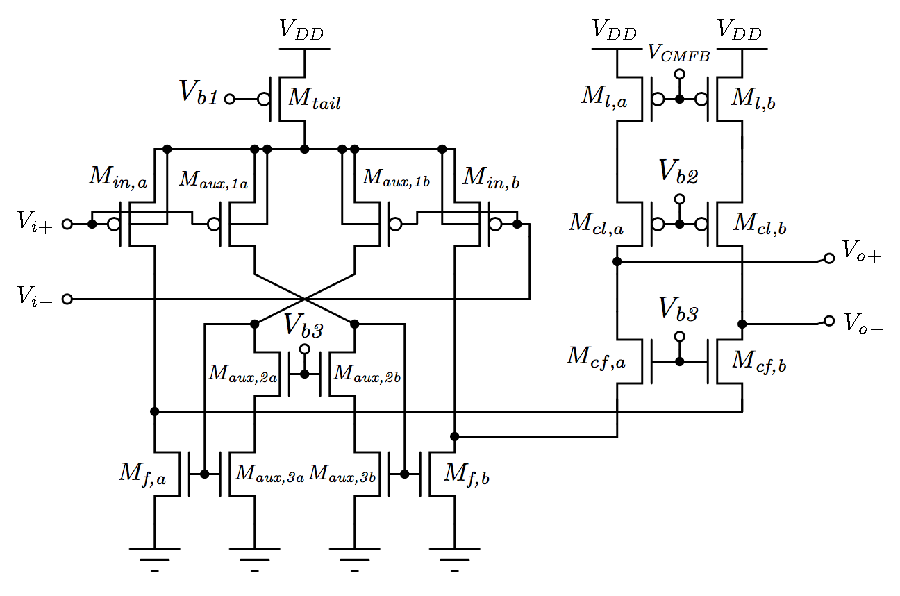
\includegraphics[width=5.5in]{./Figures/Filter/OTA_post.eps}
	\caption[Recycling folded cascode OTA schematic.]{Recycling folded cascode OTA schematic. Three terminal NMOS and PMOS devices are with their bodies tied to ground and $V_\textit{DD}$ respectively. CMFB circuit is shown in Fig.~\ref{fig:CMFB_post}}\label{fig:OTA_post}
\end{figure}
\begin{figure}[!t]
	\centering
	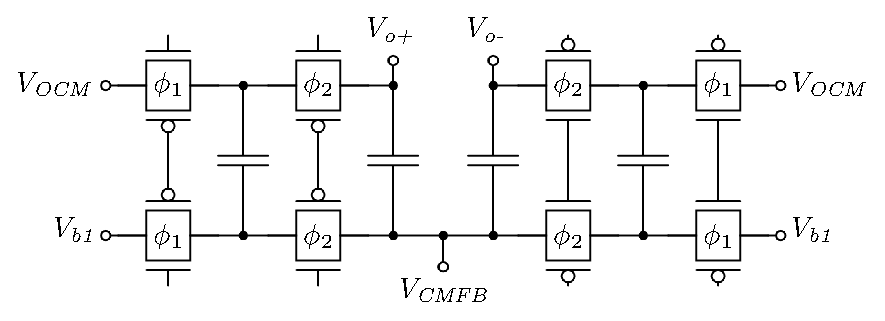
\includegraphics[width=4.6in]{./Figures/Filter/CMFB_post.eps}
	\caption{OTA discrete-time commmon-mode feedback circuit schematic.}\label{fig:CMFB_post}
\end{figure}
\begin{figure}[!t]
	\centering
	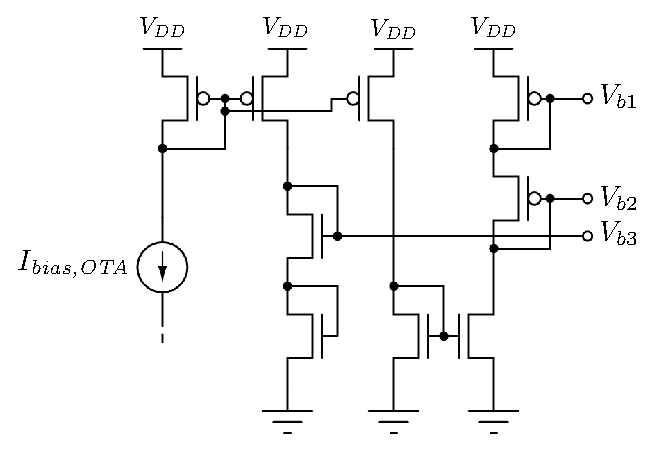
\includegraphics[width=4in]{./Figures/Filter/bias_ota_post.eps}
	\caption{OTA bias network schematic.}\label{fig:bias_ota_post}
\end{figure}
\begin{table}[!t]
	\begin{center}
		\begin{tabular}{|l|r|r|r|r|}\hline
			Transistor & Bias current & $g_m/I_D$ & $W$ & $L$ \\ \hline\hline
			$M_\text{in}$ & $51.3\,\mu\text{A}$  & $14.9\,\text{mS}/\text{mA}$  & $48\,\mu\text{m}$ & $0.36\,\mu\text{m}$ \\ \hline
			$M_\text{tail}$ & $201.7\,\mu\text{A}$  & $8.2\,\text{mS}/\text{mA}$  & $64\,\mu\text{m}$ & $0.45\,\mu\text{m}$ \\ \hline 
			$M_\text{f}$ & $100.6\,\mu\text{A}$  & $8.7\,\text{mS}/\text{mA}$  & $8\,\mu\text{m}$ & $0.45\,\mu\text{m}$ \\ \hline
			$M_\text{cf}$ & $49.3\,\mu\text{A}$  & $11.7\,\text{mS}/\text{mA}$  & $8\,\mu\text{m}$ & $0.45\,\mu\text{m}$ \\ \hline
			$M_\text{cl}$ & $49.3\,\mu\text{A}$  & $10.7\,\text{mS}/\text{mA}$  & $16\,\mu\text{m}$ & $0.3\,\mu\text{m}$ \\ \hline
			$M_\text{l}$ & $49.3\,\mu\text{A}$  & $7.6\,\text{mS}/\text{mA}$  & $32\,\mu\text{m}$ & $1\,\mu\text{m}$ \\ \hline
			$M_\text{aux,1}$ & $49.6\,\mu\text{A}$  & $15\,\text{mS}/\text{mA}$  & $48\,\mu\text{m}$ & $0.36\,\mu\text{m}$ \\ \hline
			$M_\text{aux,2}$ & $49.6\,\mu\text{A}$  & $9.5\,\text{mS}/\text{mA}$  & $2\,\mu\text{m}$ & $0.18\,\mu\text{m}$ \\ \hline
			$M_\text{aux,3}$ & $49.6\,\mu\text{A}$  & $6\,\text{mS}/\text{mA}$  & $4\,\mu\text{m}$ & $0.45\,\mu\text{m}$ \\ \hline
		\end{tabular}
		\vspace*{5pt}
		\caption{Filter OTA design values.}
		\label{tab:OTA_sizes}
	\end{center}
\end{table}

\subsection{Variable Capacitor}
Fig.~\ref{fig:cap_array_post} shows the schematic of the binary-weighted array used to implement the variable capacitor $C_S$. All capacitors $C_{S,bn}$ were designed as a parallel connection of unity metal-insulator-metal (MIM) capacitors $C_u=8.1\,\text{fF}$  (with an area of $2.7\,\micro\text{m}\times2.7\,\micro\text{m}$), which for matching purposes were also used to implement capacitor $C_F$. CMOS switches were sized to meet filter speed specifications.  Switch control signals will be directly bonded out off-chip. A \mbox{serial-programmable} memory to store the filter coefficients, and which will be connected directly to these control signals - to avoid the \mbox{unnecessary} use of IC pads -, will be included in future revisions of the Bean.

\begin{figure}[!t]
	\centering
	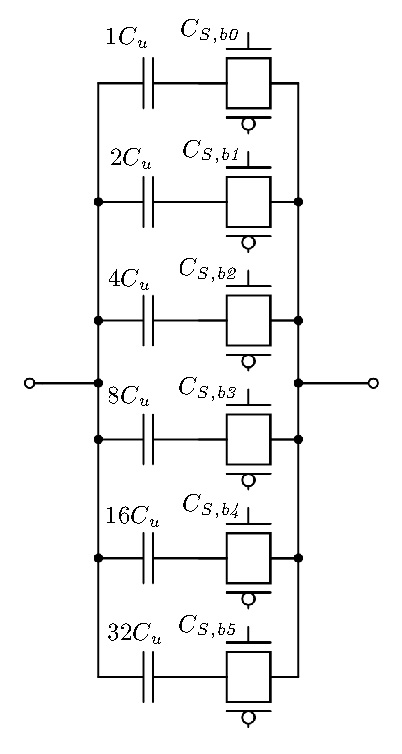
\includegraphics[width=1.8in]{./Figures/Filter/cap_array_post.eps}
	\caption{6-bit programmable capacitor.}\label{fig:cap_array_post}
\end{figure}

\subsection{Rail-to-Rail buffer}
A signal buffer is required to buffer some of the Bean prototype voltages for scope probing. The buffer must be able to drive a $8\,\text{pF}$ load at a reasonable speed and power dissipation, with truly rail-to-rail input and output voltages. Fig.~\ref{fig:buffer_post} shows the schematic of a rail-to-rail operational amplifier (op-amp) used to implement a unity-gain voltage buffer amplifier.

The two-stage op-amp consists of a rail-to-rail constant-$g_m$ input stage \citep{hogervorst101}, composed by two complementary input pairs and an electronic zener diode, $M_\text{in1}$-$M_\text{in2}$, $M_\text{ip,a}$-$M_\text{ip,b}$ and $M_\textit{zp}$-$M_\textit{zn}$,  followed by folded-cascode, current-mirroring loads, \mbox{$M_\textit{cln1}$-$M_\textit{ln1}$}, $M_\textit{cln2}$-$M_\textit{ln2}$, $M_\textit{clp1}$-$M_\textit{lp1}$ and $M_\textit{clp2}$-$M_\textit{lp2}$, and a class-AB output \citep{hogervorst102}, $M_\textit{op}$-$M_\textit{on}$. Transistors $M_\textit{sn1}$-$M_\textit{sn2}$ and $M_\textit{sp1}$-$M_\textit{sp2}$ implement a translinear loop \citep{analogessentials}, producing the voltage shifts necessary to set the output devices quiescent current consumption.

As in most of two-stage amplifiers, stability must be assured with a proper compensation scheme. In this design, capacitor $C_C$, also known as Miller capacitor, is placed to lower the frequency of the dominant pole and to increase the frequency of the secondary pole, and thus, it helps to increase the phase margin of the amplifier, while resistor $R_Z$ is used to shift to infinity the right-half plane zero that appears because adding $C_C$. Since $C_C$ is calculated as a function of the input stage's total transconductance, the constant-$g_m$ compensation technique used for the input stage helps to maintain a constant frequency response over all the input common mode range.

To assure predictable bias currents and a true rail-to-rail input and output voltage ranges, a proper bias network must be designed. Fig.~\ref{fig:bias_buffer_post} shows the schematic of the bias network used for this op-amp \citep{baker101}. All bias voltages are driven by cascoded current mirrors, which have high output resistance in order to reduce the effect of $V_{ds}$ over the mirrored current. Transistor sizes were calculated to assure a maximum amplifier output swing and mirror currents were chosen to maintain a good tradeoff between mirrored currents sensibility and bias network power consumption. 

Table~\ref{tab:buffer_sizes} shows the parameter values for the rail-to-rail buffer design. Transistor sizes were calculated with the same methodology as that used for the OTA design. SPICE simulations predict an open-loop DC gain of $103$\,dB, a crossover frequency of $52$,MHz, and a phase margin of $72\,^\circ$ measured with an $8\,\text{pF}$ load. 
\begin{table}[!t]
	\begin{center}
		\begin{tabular}{|l|r|r|r|r|}\hline
			Transistor & Bias current & $g_m/I_D$ & $W$ & $L$ \\ \hline\hline
			$M_\textit{in}$ & $10.4\,\mu\text{A}$ & $21.2\,\text{mS}/\text{mA}$ & $12.8\,\mu\text{m}$ & $0.45\,\mu\text{m}$ \\ \hline
			$M_\textit{ip}$ & $9.2\,\mu\text{A}$ & $19.4\,\text{mS}/\text{mA}$ & $40\,\mu\text{m}$ & $0.45\,\mu\text{m}$ \\ \hline
			$M_\textit{tp}$ & $60.6\,\mu\text{A}$ & $7.4\,\text{mS}/\text{mA}$ & $20\,\mu\text{m}$ & $0.45\,\mu\text{m}$ \\ \hline
			$M_\textit{tn}$ & $62.9\,\mu\text{A}$ & $9.2\,\text{mS}/\text{mA}$ & $6.4\,\mu\text{m}$ & $0.45\,\mu\text{m}$ \\ \hline
			$M_\textit{lp}$ & $26.3\,\mu\text{A}$ & $9.1\,\text{mS}/\text{mA}$ & $10\,\mu\text{m}$ & $0.45\,\mu\text{m}$ \\ \hline
			$M_\textit{clp}$ & $16\,\mu\text{A}$ & $14.2\,\text{mS}/\text{mA}$ & $20\,\mu\text{m}$ & $0.45\,\mu\text{m}$ \\ \hline
			$M_\textit{ln}$ & $25.2\,\mu\text{A}$ & $10.9\,\text{mS}/\text{mA}$ & $3.2\,\mu\text{m}$ & $0.45\,\mu\text{m}$ \\ \hline
			$M_\textit{cln}$ & $16\,\mu\text{A}$ & $16.8\,\text{mS}/\text{mA}$ & $6.4\,\mu\text{m}$ & $0.45\,\mu\text{m}$ \\ \hline
			$M_\textit{op}$ & $282\,\mu\text{A}$ & $9\,\text{mS}/\text{mA}$ & $100\,\mu\text{m}$ & $0.45\,\mu\text{m}$ \\ \hline
			$M_\textit{on}$ & $282\,\mu\text{A}$ & $10.7\,\text{mS}/\text{mA}$ & $32\,\mu\text{m}$ & $0.45\,\mu\text{m}$ \\\hline
		\end{tabular}
		\vspace*{5pt}
		\caption{Rail-to-rail buffer main design values.}
		\label{tab:buffer_sizes}
	\end{center}
\end{table}
\begin{figure}[!t]
	\centering
	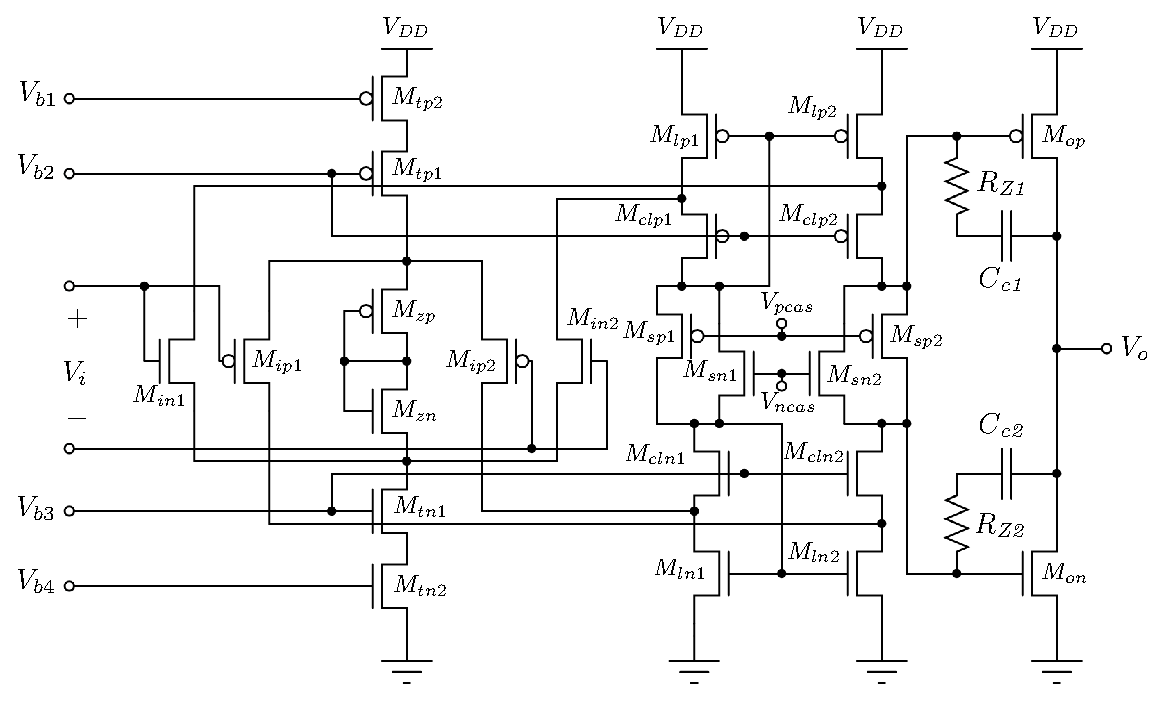
\includegraphics[width=6in]{./Figures/Filter/buffer_post.eps}
	\caption{Rail-to-rail operational amplifier schematic.}\label{fig:buffer_post}
\end{figure}
\begin{figure}[!t]
	\centering
	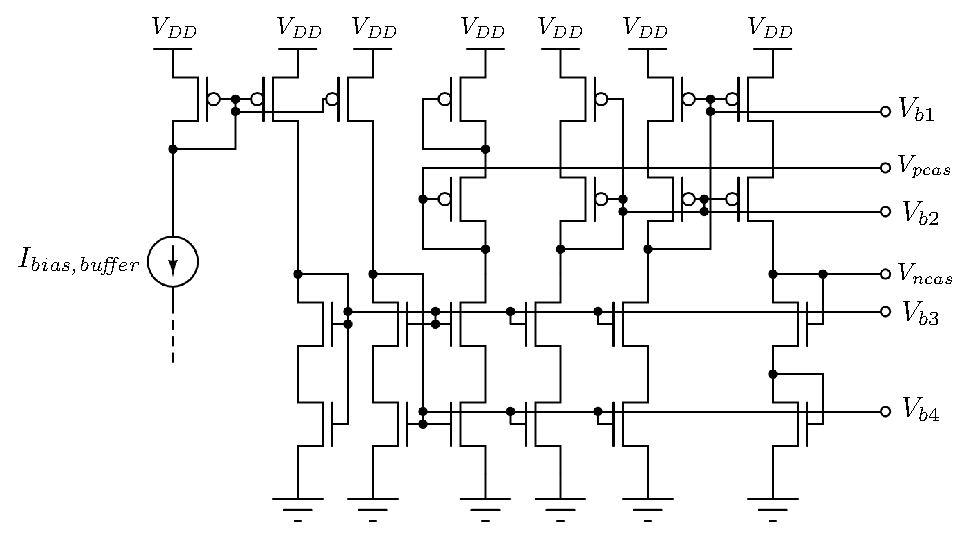
\includegraphics[width=5in]{./Figures/Filter/bias_buffer_post.eps}
	\caption{Op-amp bias network schematic.}\label{fig:bias_buffer_post}
\end{figure}


\subsection{IC bias network}
The previous version of the Bean uses a voltage distribution scheme to bias all the circuits in the IC, but it can cause big problems due to IR drop and process gradients, so a more common current distribution scheme was chosen for this iteration of the design \citep{murmann101}.  The main disadvantage of this architecture is the additional current consumption, but this drawback is marginal compared to the entire IC power budget and the obtained benefits. To achieve a good power supply rejection (PSR), a supply-insensitive bias network was chosen to implement the global bias cell, from which all the bias currents are generated. Fig.~\ref{fig:bias_all_post} shows a diagram of the current distribution bias scheme. For simplicity, only three current branches are illustrated, although five were used in the final design. Fig.~\ref{fig:bias_filter_post} shows the schematic of a $\beta$-multiplier bias circuit, the architecture selected to implement the supply-insensitive bias network. This consist of a \mbox{self-biased} \mbox{current-reference} network, a \mbox{start-up} circuit, because there are two possible operating points, and a cascode current mirror. The $\beta$-multiplier is an example of a circuit that uses positive feedback. The addition of the resistor kills the closed loop gain\footnote{A positive feedback system can be stable if its closed loop gain is less than one.}. However, if the parasitic capacitance of this resistor is large, it will increase the loop gain and push the feedback system closer to instability. If the resistor, for example, is bonded out off-chip to set the current, it is likely that this bias circuit will oscillate \citep{baker101}.

\begin{figure}[!t]
	\centering
	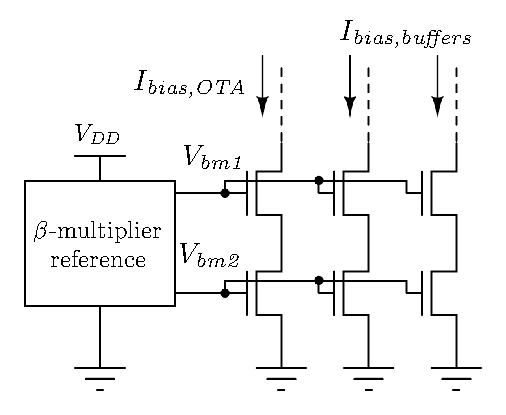
\includegraphics[width=3in]{./Figures/Filter/bias_all_post.eps}
	\caption{Current distribution bias scheme.}\label{fig:bias_all_post}
\end{figure}
\begin{figure}[!t]
	\centering
	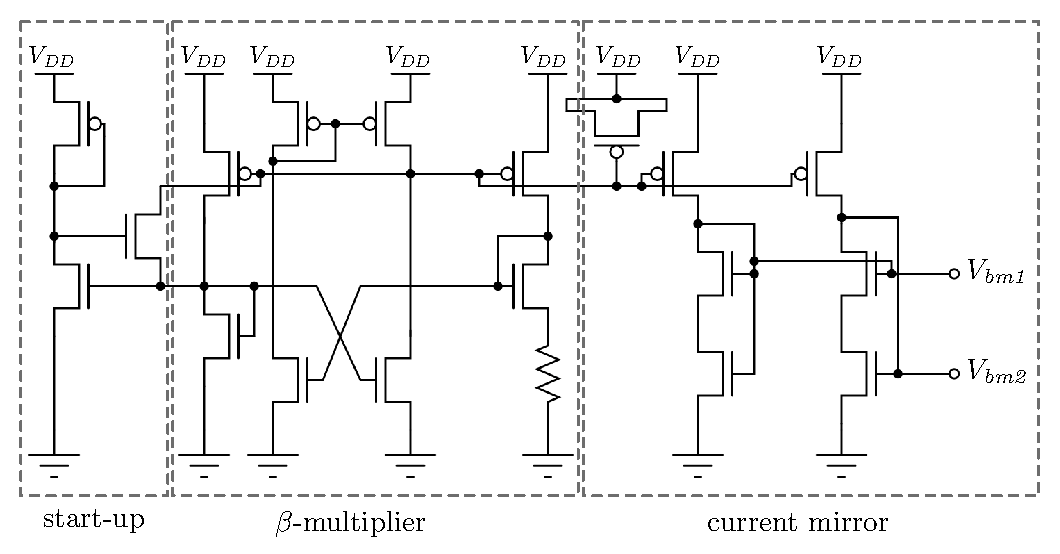
\includegraphics[width=6in]{./Figures/Filter/bias_filter_post}
	\caption{$\beta$-multiplier bias schematic.}\label{fig:bias_filter_post}
\end{figure}